 \begin{figure}[htb]
 
  \centering
  \begin{tabular}{  c p{0.7cm} c}
    %\centering
    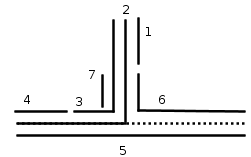
\includegraphics[width=5cm]{img/noClaw365.png} & &
    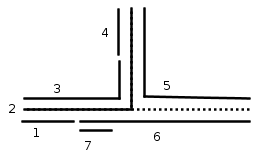
\includegraphics[width=5.2cm]{img/noClaw356.png}
    \\
    \footnotesize %\centering 
    (a)  \footnotesize Claw-clique $P_3$, $P_6$, $P_5$ && \footnotesize (b) Claw-clique $P_3$, $P_5$, $P_6$\\
    \multicolumn{3}{c}{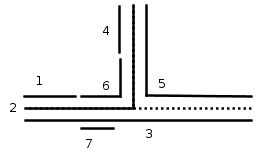
\includegraphics[width=5cm]{img/noClaw653.png}  }
    \\
    \multicolumn{3}{c}{ \footnotesize (c) Claw-clique $P_6$, $P_5$, $P_3$ }
    \\
  \end{tabular}
 
%  \center%6.3
%  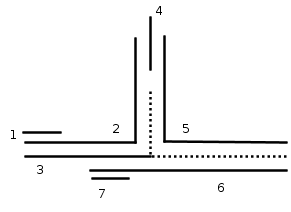
\includegraphics[width=5cm]{./img/noClaw256.png}
 \caption{Constructions in single bend of $k$-tent with $P_3$, $P_5$ and $P_6$ in claw-clique representation }
\label{fig:noClaw365}
\end{figure}  
 